\documentclass[11pt,a4paper]{article}

\usepackage[utf8]{inputenc}
\usepackage[T1]{fontenc}
\usepackage[margin=2.5cm]{geometry}
\usepackage{booktabs}
\usepackage{xcolor}
\usepackage{graphicx}
\usepackage{hyperref}
\usepackage{parskip}

\hypersetup{colorlinks=true, linkcolor=black, urlcolor=blue}

\newcommand{\unk}{\textcolor{gray}{UNKNOWN}}

\title{\textbf{Real-World Spectra Test Across All Trained Model Families}\\
\large CNNIRPLASTICS --- FTIR Polymer Classification}
\author{Jose Maria Contreras Prada}
\date{12 June 2026}

\begin{document}
\maketitle

\begin{abstract}
This report documents the work performed on 12 June 2026: (1) integration of the
\texttt{add-cosine-baseline-eval} and the new \texttt{experiments} branches into
\texttt{external-dataset-eval}, bringing the full staged-experiment pipeline and
all trained model artifacts into one branch; and (2) a blind test of 30 newly
measured real-world FTIR spectra against \emph{every} trained model family in
the repository, including per-sample saliency maps (gradient saliency and 1-D
Grad-CAM) for the deployment CNN ensemble. The deployment configuration
(random-forest soft-vote with a 0.89 reject gate) accepted only 4 of the 30
samples --- \texttt{ldpewet}$\to$HDPE, \texttt{pvcscrepe}$\to$PVC,
\texttt{wetcd}$\to$PS --- and rejected every clear non-plastic, while the
uncalibrated CNN softmax assigned 100\% confidence to several out-of-distribution
materials. The gate also rejected several plausible plastics (wet PP, LDPE-like
films) on which all four modern model families agreed, suggesting the 0.89
threshold is conservative for spectra from this instrument.
\end{abstract}

\section{Branch integration}

The session started by synchronising the local repository with
\texttt{origin}. Two lines contained new work relative to
\texttt{external-dataset-eval}:

\begin{itemize}
  \item \textbf{\texttt{add-cosine-baseline-eval}} (7 commits): SLOPP and
        SLOPP-E reference datasets as CSV, a FLOPP dataset builder, and the
        class-set cleanup commits.
  \item \textbf{\texttt{experiments}} (2 commits, new branch): the staged
        experiment package \texttt{experiments/} (stage 1 data summary, stage 2
        RF preprocessing sweep, stage 3 CNN/RF head-to-head, stage 4
        stress/OOD testing), the full \texttt{experiments\_output/} artifact
        tree with all trained models, cached aligned matrices, results JSON,
        figures, and \texttt{FINAL\_REPORT}.
\end{itemize}

Both were merged into \texttt{external-dataset-eval} without conflicts
(merge commits \texttt{0f1224f} and \texttt{77b852b}); \texttt{origin/main} and
\texttt{origin/restructure} contained nothing new. The branch was pushed back
to GitHub at the end of the session (\texttt{428a2dc}).

\section{Model inventory}

Every saved, loadable model family in the repository was tested
(table~\ref{tab:models}). The two \emph{legacy} families predate the
experiments pipeline; the four modern families come from the merged
\texttt{experiments} branch. The \emph{deployment} configuration, as specified
in \texttt{experiments\_output/models/final/deployment.json}, is the
random-forest 5-fold soft-vote with a reject rule: if the maximum class
probability is below 0.89 the sample is declared UNKNOWN.

\begin{table}[h]
\centering
\scriptsize
\setlength{\tabcolsep}{4pt}
\begin{tabular}{lllll}
\toprule
Family & Location & Models & Input grid & Preprocessing \\
\midrule
legacy-cnn & \texttt{output/} & 4 CNN folds & 1868 pts & smooth+asls+snv \\
legacy-rf  & \texttt{output/} & 5 RF folds  & 600 pts  & smooth+asls+snv \\
final-rf   & \texttt{models/final/} & 5 RF folds (+\texttt{rf\_final}) & 1868 pts & snv, reject@0.89 \\
final-cnn  & \texttt{models/final/} & 5 CNN folds & 1868 pts & snv \\
cnn-d1     & \texttt{models/no\_os\_\_smooth+d1+snv/} & 5 CNN folds & 1868 pts & smooth+d1+snv \\
cnn-os     & \texttt{models/with\_os\_\_norm-snv/} & 5 CNN folds & 395 pts (804--3168\,cm$^{-1}$) & snv \\
\bottomrule
\end{tabular}
\caption{All tested model families. ``Location'' paths under
\texttt{experiments\_output/} where applicable. All families output the six
commodity classes HDPE, LDPE, PP, PS, PVC, PET.}
\label{tab:models}
\end{table}

The Keras models were trained on Google Colab with a newer Keras version; a
compatibility shim (stripping the unknown \texttt{quantization\_config} layer
kwarg, as already used in \texttt{scripts/saliency\_cnn.py}) is required to
load them locally and is included in the test script.

\section{Test data and method}

Thirty spectra measured on the lab FTIR were provided as two-column
JCAMP-style text files (wavenumber in cm$^{-1}$, intensity in \%T;
2{,}521 points from $\sim$400 to $\sim$4000\,cm$^{-1}$). The set deliberately
mixes plastics, suspected bioplastics (black/grey printed ``pla'' samples),
wet samples, and clear non-plastics (aluminium, paper, textile, rubber bands,
a snack wrapper, the instrument background scan, thermoplastic polyurethane).

The pipeline implemented in \texttt{scripts/test\_lab\_downloads.py}:

\begin{enumerate}
  \item parse each file, skipping \texttt{\#\#} header lines;
  \item align each spectrum to each family's wavenumber grid by linear
        interpolation with edge clamping (the convention used for all
        external evaluations in the repo);
  \item apply that family's exact training preprocessing
        (per-spectrum, leakage-free: SNV, or smooth+AsLS+SNV, or
        smooth+1st-derivative+SNV);
  \item soft-vote the fold ensemble of each family;
  \item apply the deployment reject rule to the final-rf probabilities;
  \item compute per-sample explainability maps for the deployment CNN
        ensemble: vanilla gradient saliency
        $|\partial p_{\hat c}/\partial x|$ and 1-D Grad-CAM on the last
        convolutional layer, averaged over the five folds, for the predicted
        class $\hat c$.
\end{enumerate}

\section{Results}

Table~\ref{tab:preds} gives every prediction. The deployment model accepted
\textbf{4 of 30} samples and declared the remaining 26 UNKNOWN.

\begin{table}[p]
\centering
\scriptsize
\setlength{\tabcolsep}{4pt}
\begin{tabular}{llllllll}
\toprule
File & \textbf{Deployment} & legacy-cnn & legacy-rf & final-rf & final-cnn & cnn-d1 & cnn-os \\
\midrule
allumium          & \unk & PVC 100\% & PP 31\%  & PVC 60\% & PVC 47\%  & PVC 100\% & PET 73\% \\
background        & \unk & HDPE 100\%& HDPE 26\%& PVC 54\% & PVC 100\% & PVC 100\% & PET 83\% \\
blaclpla          & \unk & PVC 75\%  & PP 30\%  & PET 37\% & PS 50\%   & HDPE 55\% & PS 60\% \\
blaclpla2         & \unk & PVC 75\%  & PP 31\%  & PET 37\% & PVC 55\%  & HDPE 72\% & PS 60\% \\
blaclpla3         & \unk & PVC 75\%  & PP 30\%  & PET 37\% & PVC 57\%  & HDPE 39\% & PS 60\% \\
brown             & \unk & PVC 78\%  & PP 24\%  & PVC 67\% & HDPE 100\%& HDPE 79\% & HDPE 70\% \\
brown2            & \unk & PVC 82\%  & PP 24\%  & PVC 67\% & HDPE 99\% & HDPE 82\% & HDPE 51\% \\
greypla           & \unk & PVC 75\%  & PP 30\%  & PET 37\% & PVC 52\%  & HDPE 76\% & PS 60\% \\
greypla2          & \unk & PVC 75\%  & PP 32\%  & PET 37\% & PVC 60\%  & PET 41\%  & PS 60\% \\
greypla3          & \unk & PVC 75\%  & PP 31\%  & PET 37\% & PVC 59\%  & HDPE 74\% & PS 59\% \\
greypla4          & \unk & PVC 75\%  & PP 30\%  & PET 37\% & PVC 59\%  & HDPE 45\% & PS 59\% \\
ldpewet           & \textbf{HDPE} & PET 41\% & PS 25\% & HDPE 96\% & HDPE 100\% & HDPE 67\% & HDPE 79\% \\
orangerubberband  & \unk & PVC 100\% & PP 26\%  & PP 77\%  & PP 100\%  & PP 100\%  & PP 98\% \\
orangerubberband2 & \unk & PVC 100\% & PP 33\%  & PP 77\%  & PP 100\%  & PP 76\%   & PP 99\% \\
oreo              & \unk & PVC 100\% & PP 37\%  & PVC 64\% & PVC 100\% & PVC 100\% & PP 43\% \\
oreo2             & \unk & PVC 100\% & PP 37\%  & PVC 62\% & PVC 88\%  & PVC 100\% & PVC 50\% \\
paper1            & \unk & PVC 74\%  & PET 33\% & PVC 73\% & HDPE 78\% & PVC 58\%  & HDPE 96\% \\
pop               & \unk & PET 50\%  & HDPE 28\%& LDPE 76\%& LDPE 100\%& LDPE 100\%& LDPE 98\% \\
pop2              & \unk & PET 53\%  & HDPE 28\%& LDPE 80\%& LDPE 100\%& LDPE 100\%& LDPE 97\% \\
pvcscrepe         & \textbf{PVC} & PVC 100\% & PP 37\% & PVC 92\% & PVC 100\% & PVC 100\% & PVC 100\% \\
TPU               & \unk & PVC 100\% & HDPE 27\%& PET 45\% & PET 37\%  & PVC 61\%  & PET 96\% \\
TPU2              & \unk & PVC 100\% & HDPE 26\%& PET 45\% & PVC 38\%  & PVC 62\%  & PET 95\% \\
TPU3              & \unk & PVC 100\% & HDPE 27\%& PET 44\% & PS 35\%   & PVC 68\%  & PET 97\% \\
wetcd             & \textbf{PS} & PVC 54\% & PP 31\% & PS 89\% & PS 100\% & PS 100\% & PS 100\% \\
wetpla            & \unk & PVC 75\%  & PP 31\%  & PET 32\% & PVC 79\%  & HDPE 94\% & PS 51\% \\
wetpp             & \unk & PVC 34\%  & HDPE 24\%& PP 69\%  & PP 96\%   & PP 100\%  & PP 87\% \\
whitetextile      & \unk & HDPE 75\% & PP 25\%  & PVC 61\% & HDPE 100\%& HDPE 59\% & HDPE 69\% \\
whitetextile2     & \unk & HDPE 100\%& PET 22\% & PVC 61\% & HDPE 100\%& HDPE 68\% & HDPE 56\% \\
yellowpap         & \unk & HDPE 100\%& PP 25\%  & PP 57\%  & PP 81\%   & PP 100\%  & PP 96\% \\
yellowpapturned   & \unk & PVC 100\% & HDPE 27\%& PVC 58\% & PVC 98\%  & PVC 100\% & PVC 99\% \\
\bottomrule
\end{tabular}
\caption{Every model family on every spectrum: predicted class and ensemble
confidence. \textbf{Deployment} = final-rf soft-vote with the 0.89 reject
gate from \texttt{deployment.json}.}
\label{tab:preds}
\end{table}

\subsection{Accepted samples}

\begin{itemize}
  \item \texttt{ldpewet} $\to$ \textbf{HDPE} (RF 96\%, CNN 100\%). A wet LDPE
        sample landing on HDPE is the familiar polyethylene-pair confusion;
        the density-related band differences (1377\,cm$^{-1}$ branch methyl,
        730/719 split) are subtle and easily masked by water.
  \item \texttt{pvcscrepe} $\to$ \textbf{PVC} (RF 92\%; all four modern
        families 100\%). The saliency map (figure~\ref{fig:pvc}) shows the
        ensemble keying on the $\sim$615\,cm$^{-1}$ C--Cl stretch region and
        the 1250--1430\,cm$^{-1}$ CH$_2$ deformation bands --- chemically the
        right evidence.
  \item \texttt{wetcd} $\to$ \textbf{PS} (RF 89\%, CNN 100\%). Correct if the
        measured surface was the jewel case (polystyrene); the disc itself is
        polycarbonate, which is outside the six-class scope.
\end{itemize}

\subsection{Out-of-distribution behaviour}

Every clear non-plastic was rejected: aluminium, the background scan, paper,
textiles, rubber bands, the snack wrapper, and all three TPU measurements.
This matters because the CNN softmax alone was \emph{confidently wrong} on
several of them --- \texttt{background} $\to$ PVC at 100\%, \texttt{oreo}
$\to$ PVC at 100\%, \texttt{whitetextile} $\to$ HDPE at 100\% --- reproducing
on fresh data the calibration warning recorded in \texttt{deployment.json}
(CNN reject AUROC 0.836, softmax not usable as confidence). The TPU spectra
produced maximally diffuse predictions across all families (35--45\%),
textbook OOD behaviour. The black and grey printed samples
(\texttt{blaclpla*}, \texttt{greypla*}, \texttt{wetpla}) drew low-confidence,
mutually contradictory predictions from every family (PVC $\sim$55\% / PS
60\% / HDPE 40--90\%); if these are PLA prints the rejection is correct, and
carbon-black-filled samples also genuinely yield washed-out ATR spectra.

\subsection{Borderline rejections}

The gate also rejected samples that look like genuine commodity plastics on
which all four modern families agree:

\begin{itemize}
  \item \texttt{wetpp} $\to$ PP (CNN 96\%, d1-CNN 100\%, OS-CNN 87\%) but RF
        only 69\%;
  \item \texttt{pop}/\texttt{pop2} $\to$ LDPE (three CNN families
        97--100\%) but RF 76--80\%;
  \item \texttt{yellowpapturned} $\to$ PVC at 98--100\% on three families
        (likely the coating/laminate side of the paper), RF 58\%.
\end{itemize}

Wet or contaminated surfaces depress the RF vote below 0.89, so the
deployment threshold --- tuned on FLOPP-e/BLoP --- trades these away. If
ground truth can be confirmed for these files, this set is a natural
calibration set for re-tuning the threshold to this instrument.

\subsection{Legacy models}

The legacy families are not usable on this data. The legacy CNN collapses to
PVC at $\sim$100\% for most inputs regardless of content, and the legacy RF
never exceeds 37\% confidence (it expects a different 600-point grid and an
older training distribution). The retraining done in the
\texttt{experiments} branch was clearly worthwhile.

\section{Saliency maps}

For each sample, gradient saliency and 1-D Grad-CAM were computed for the
deployment CNN ensemble's predicted class and overlaid on the preprocessed
spectrum (folder \texttt{saliency/} next to this report). Figure
\ref{fig:overview} stacks all 30 Grad-CAM profiles.

\begin{figure}[p]
  \centering
  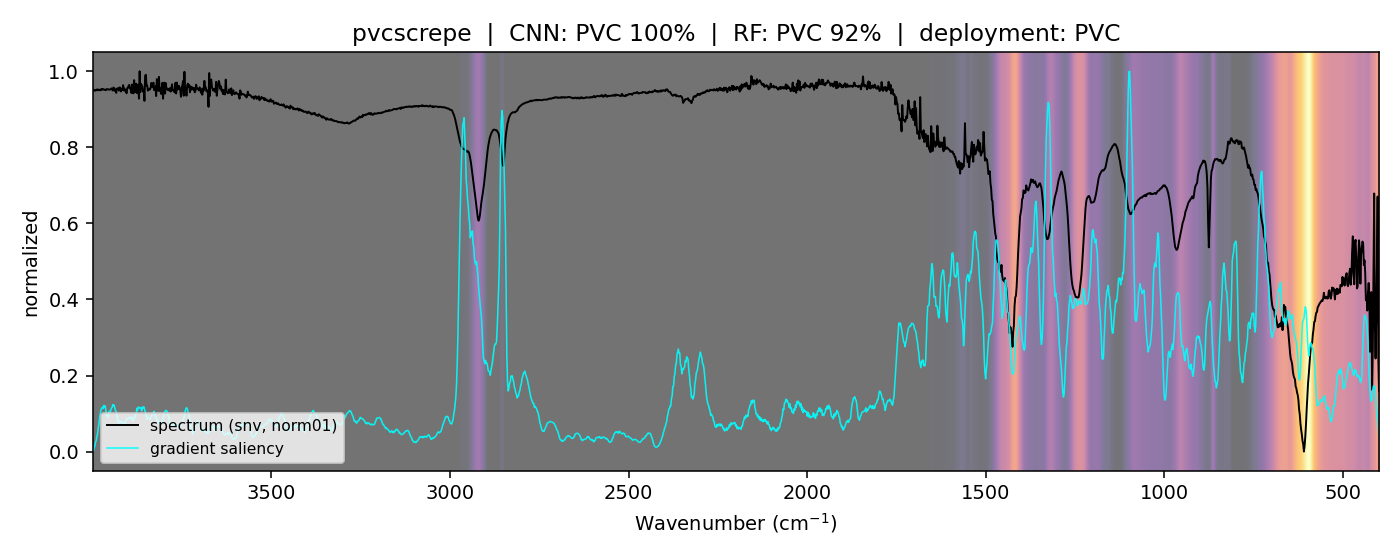
\includegraphics[width=\textwidth]{saliency/pvcscrepe.png}
  \caption{\texttt{pvcscrepe}: attention concentrates on the C--Cl stretch
  region ($\sim$615\,cm$^{-1}$) and the 1250--1430\,cm$^{-1}$ bands ---
  genuine PVC evidence.}
  \label{fig:pvc}
\end{figure}

\begin{figure}[p]
  \centering
  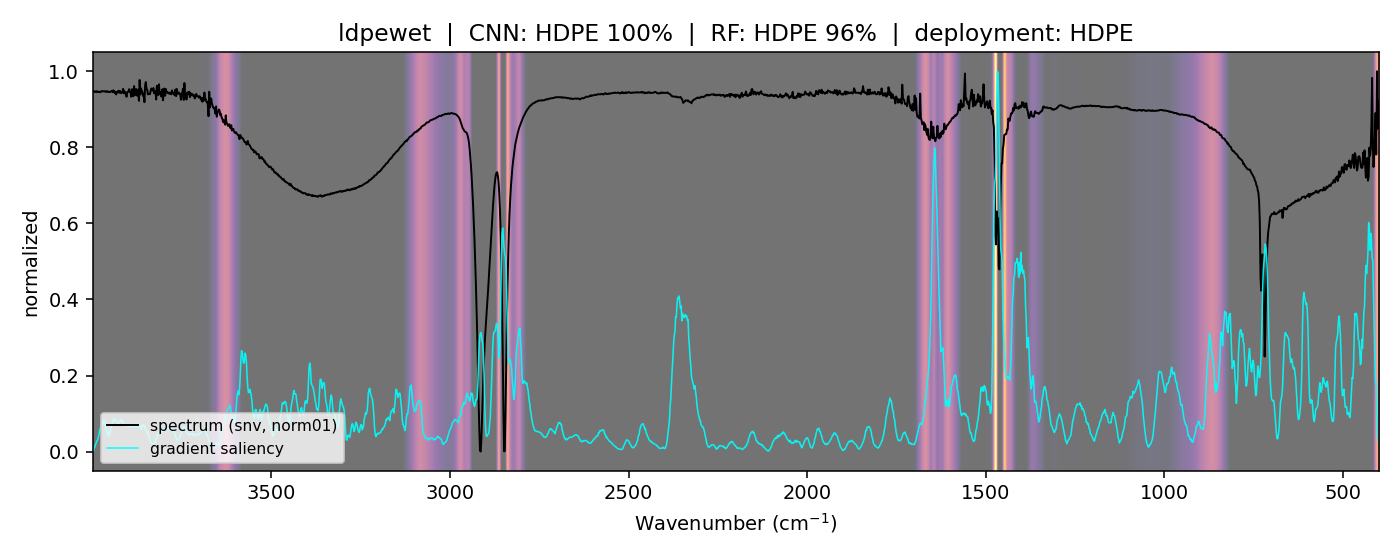
\includegraphics[width=\textwidth]{saliency/ldpewet.png}
  \caption{\texttt{ldpewet} (accepted as HDPE): weight on the CH$_2$
  stretch/bend regions shared by both polyethylenes; the discriminating
  LDPE features are weak, consistent with the HDPE/LDPE swap.}
  \label{fig:ldpe}
\end{figure}

\begin{figure}[p]
  \centering
  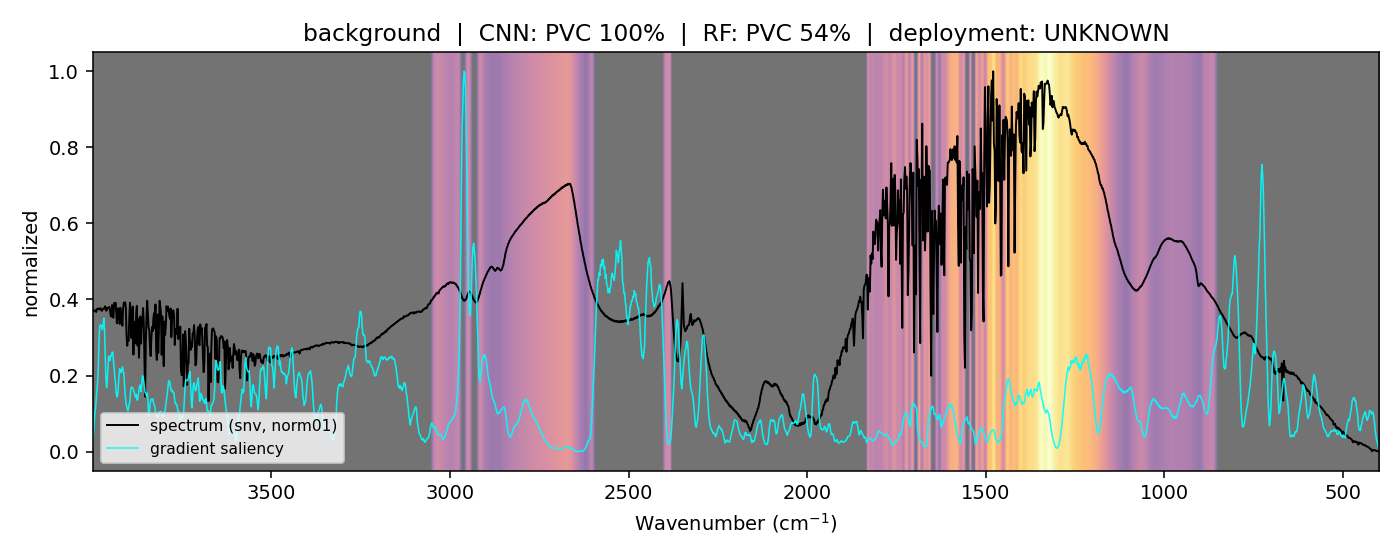
\includegraphics[width=\textwidth]{saliency/background.png}
  \caption{\texttt{background} (instrument background scan): the CNN reports
  PVC at 100\% while attending to broad, featureless regions --- a clear
  illustration of why the uncalibrated softmax must sit behind the RF reject
  gate.}
  \label{fig:bg}
\end{figure}

\begin{figure}[p]
  \centering
  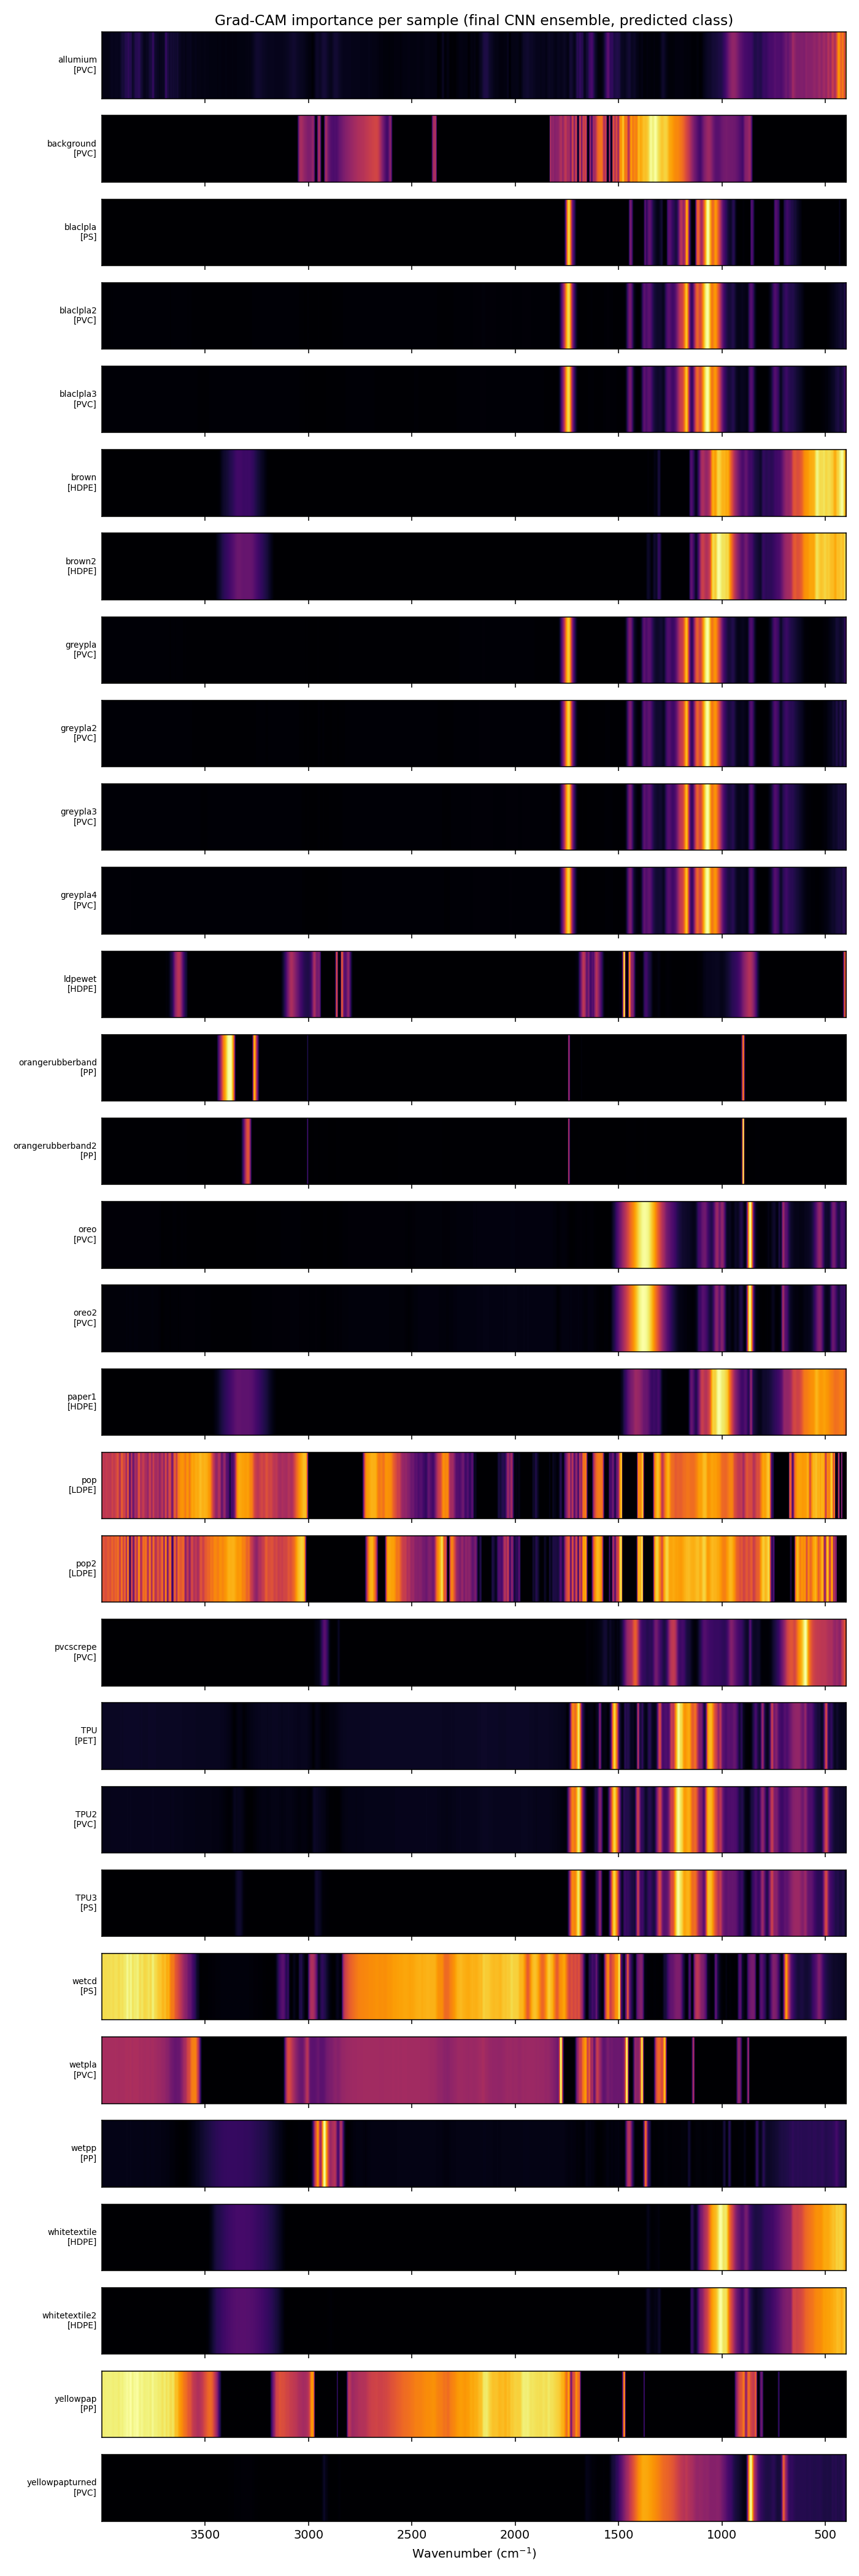
\includegraphics[width=\textwidth]{saliency_overview.png}
  \caption{Grad-CAM importance for all 30 samples (deployment CNN ensemble,
  predicted class). Accepted samples show localized, band-aligned attention;
  rejected OOD samples tend to show diffuse or baseline-dominated attention.}
  \label{fig:overview}
\end{figure}

\section{Conclusions and next steps}

\begin{enumerate}
  \item The merged deployment pipeline behaves as designed on completely fresh
        real-world data: it never produced a confident wrong answer, at the
        cost of high abstention (26/30 UNKNOWN).
  \item The CNN softmax over-confidence on OOD inputs is reproduced
        (100\% on a background scan); the RF gate is what makes the system
        safe.
  \item The 0.89 threshold appears too strict for wet/contaminated samples
        from this instrument; \texttt{wetpp}, \texttt{pop}, and
        \texttt{yellowpapturned} are candidates for threshold re-calibration
        once their ground truth is confirmed.
  \item The legacy \texttt{output/} models should be considered deprecated
        for evaluation purposes.
  \item All artifacts are committed on \texttt{external-dataset-eval}
        (\texttt{428a2dc}): the test script
        \texttt{scripts/test\_lab\_downloads.py}, the prediction tables, and
        all 30 saliency maps.
\end{enumerate}

\end{document}
